\chapter{Link Layer Security}

Link Layer Security, or LLSEC, is a security measure that implements cryptography just above the physical layer.

Introducing cryptography at a lower level has several benefits. Firstly, more data being encrypted reduces the observable packet features to an adversary, such as SRC\footnote{Source Address} and DST\footnote{Destination Address} field in the IP header which are very likely to be exploited by the adversary. Secondly, authentication at lower level also prevents an active adversary from joining the network which therefore weakens his power. 

Imposing cryptography at a lower level also brings more challenge to the design of sensor network architecture. The first problem is its overhead. Even for a node that only tries to retransmits the packet to its next hop, it must decrypt the whole packet to extract its routing information, and then re-encrypt it before retransmission. This is particularly problematic in a mesh wireless sensor network as it could potentially lead to performance and energy consumption problems. Key management is also challenging due to the lossy and power optimised nature of wireless sensor network.

It is also noticeable that some packet features are not hidden even with LLSEC enabled, such as packet length, timing information and part of the MAC header.

\section{802.15.4 Security: {\it noncoresec}} \label{sec: noncoresec}
{\it noncoresec}\cite{LLSEC} is the current implementation of LLSEC in Contiki. It corresponds to the AES\_CCM\_16 ciphersuite in 802.15.4 standard. This section briefly describes how it works.

\begin{itemize}
\item {\bf Key Management}: All nodes share a network wide AES key for both encryption and authentication. The key is hardcoded during the setup stage.

\item{\bf AEAD\footnote{Authenticated Encryption with Associated Data}}: {\it noncoresec} implements AES\_CCM\_16 \footnote{CCM mode of AES-128 with 16 bytes MAC} as described in 802.15.4\cite{802154}. CCM mode turns AES into a stream cipher. The same key is used for both encryption and authentication.

\item{\bf Initial Vector (IV, or nonce)}: The IV for each packet is constructed from certain fields of unencrypted MAC frame header and therefore is public.
\end{itemize}

An adversary without the knowledge cannot join the sensor network as he cannot sent out a valid RPL message.

\section{Weak IV}

\begin{table}
\centering
\begin{tabular}{| l | l | l | l | l |}
\hline
Flags(1) & Addresses(8) & Frame Counter(4) & Security Level(1) & Block Counter(2)       \\ \hline
\end{tabular}
\caption{IV of 802.15.4 Frame with Security} \label{Tbl: 802154 Frame}
\end{table}

One problem within the {\it noncoresec} implementation is the low variance of IV. The IV is a $16$ byte bit-string constitutes of the following fields(\Cref{Tbl: 802154 Frame}):
\begin{itemize}
\item {\bf Flags (1 byte)}: This field contains part of the MAC frame header. It is identical to most (basically all) of the data packets.

\item{\bf Source Address (8 bytes)}: This is mapped from the source address field of the frame.

\item{\bf Frame Counter (4 bytes)}: This field increases by 1 for each frame sent.

\item{\bf Security Level (1 byte)}: This field indicates which ciphersuite to be used for this frame. In the case of AES\_CCM\_16, this is constantly 0x7.

\item{\bf Block Counter (2 bytes)}: This field begins from 0x0 and increases by 0x1 for each block in CCM mode. The block length for AES-128 is 16 bytes. The 2 bytes counter is sufficient as it supports up to $2^{32}$ bytes of data whereas the minimum MTU\footnote{Maximum Transmit Unit, simply speaking this is the maximum length of a packet.} required by 6lowPAN standard\cite{rfc4944} is $127$ bytes.
\end{itemize}

In the current {\it noncresec} implementation, \textbf{Flags} and \textbf{Security Level} are constant. \textbf{Block Counter} always begins from 0x0 and the \textbf{Source Address} is also constant for a specific device. Such design leaves the 4 bytes \textbf{Frame Counter} the only field that is variable. This indicates that only $2^32$ messages are allowed which is cryptographically considered to be inappropriate.

\subsection{Reset Problem}
The low variance of IV leads to a plaintext leakage problem which only requires the adversary to reboot the target node. 

The idea is that rebooting the device resets the \textbf{Frame Counter} to 0x0; hence once a pair of packets with same \textbf{Frame Counter} is found, the difference of their plaintext can be computed by their ciphertext:
\begin{equation*}
\Delta p = c_1 \oplus c_2
\end{equation*}
where $\Delta p$ is the difference of plaintexts. $c_1$ and $c_2$ are their ciphertext respectively.

\begin{example}
\begin{figure}
\centering
{
	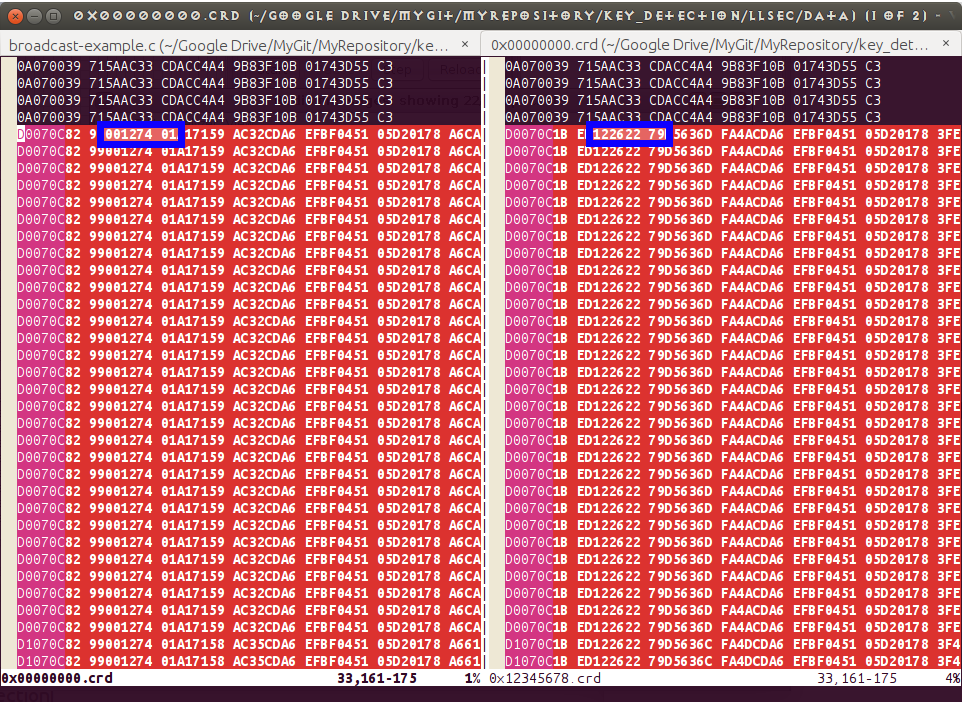
\includegraphics[width=0.9\textwidth,]{fig/resetproblem.png} 
}
\caption{Captured packets with {\it noncoresec} enabled} \label{Fig: reset problem}
\end{figure}

\Cref{Fig: reset problem} demonstrates some packet captured\footnote{The duplicated packets are caused by the retransmission of ContikiMAC\cite{ContikiMAC}.} with {\it noncoresec} enabled. These packets are captured with a sensor broadcasting a 4 byte integer with left side of \Cref{Fig: reset problem} being $[00000000]_{16}$ and right $[12345678]_{16}$. Marked are the corresponding ciphertexts which are $[00127401]_{16}$ and $[12262279]_{16}$ respectively.

As we can see, the difference of ciphertext is exactly the difference of plaintext:
\begin{equation}
\Delta p = [00127401]_{16} \oplus [12262269]_{16} = [12345678]_{16}
\end{equation}
\end{example}

\section{Distinctive packet length for RPL packets}
Some RPL packets are shorter than the minimum length of data packets which can be used to distinguish the packets.

\section{Performance issue}
The header overhead with LLSEC enabled is 20 bytes which is relatively a large overhead comparing to the 127 bytes MTU requirement of 6LowPAN standard\cite{rfc4944}.